\begin{question}
\label{ex:greedy_pig}
The Greedy Pig Game is a simple dice game. It is played with one single dice and the goal is to reach 100 points. Each player in turn start to roll the dice, if a 2-6 the corresponding points are acquired and the player can continue to roll or can stop. If a 1 is rolled the player scores a 0 and her turn ends.

Find the expected number of points for each roll.

Imagine a player that has collected $k$ points. Compute and draw the expected points obtained with a further roll. What can be concluded from this plot ?
\end{question}

\cprotEnv\begin{solution}
\begin{ipython}
ex_roll = 0
for i in range(2, 7):
    ex_roll += 1/6*i

print (ex_roll)
\end{ipython}
\begin{ioutput}
3.3333333333333
\end{ioutput}

\begin{ipython}
from matplotlib import pyplot as plt

exps = []
for k in range(1, 51):
    exp = -k*1/6
    for i in range(2, 7):
        exp += 1/6*i
    exps.append(exp)

fig = plt.figure(figsize=(10,8))
plt.plot(range(1, 51), exps)
plt.grid(True)
plt.xlabel("current turn points ($k$)")
plt.ylabel("expected points next roll")
plt.show()
\end{ipython}

Figure~\ref{fig:greedy_pig_expec} shows the distribution of the expected points in the next turn as a function of the current player points. It looks like that when the player has more than 20 points the expectation becomes negative, so it is not anymore convenient to keep rolling. This is a fundamental clue to derive a game strategy: keeps rolling until you reach 20.

\begin{figure}[htbp]
	\begin{center}
		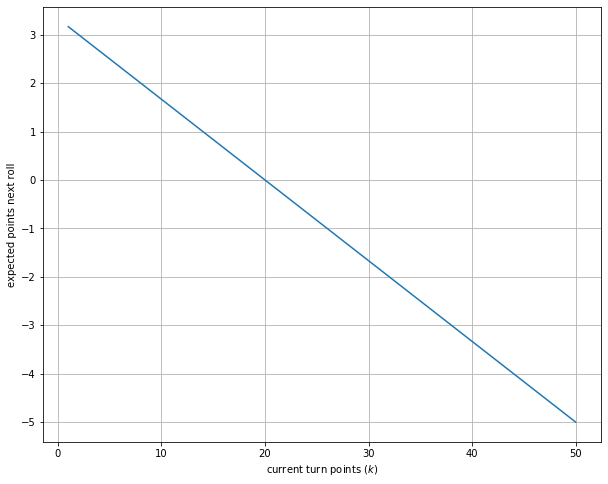
\includegraphics[width=0.7\linewidth]{figures/greedy_pig_expectation}
	\end{center}
\label{fig:greedy_pig_expec}
\end{figure}
\end{solution}
